%EXP

\subsection{Experimental Setup}

The 218 publicly-available and labeled patients were downloaded from NCBI and converted to FASTQ format using the SRA toolkit, and labeled according to the labels on EBI, as described in the Materials section. The data was split evenly into training and test sets, with each containing 109 patients. The training set had 54 T2D patients and 55 control patients, while the test set had 53 T2D patients and 56 control patients. Each read was assembled with SOAPdenovo2, with the k-mer length set to 51, reads cut off after 100 base pairs (original length of 180 base pairs), and the average insert size set to 350 in accordance with the reported average insert size reported in the MGWAS study \cite{qin041012}. Assembly for each file took 7-30 minutes, depending on the file size, and each patient was assembled in parallel. Combining the files into one file took 12 minutes. Assembly was used for all of the classification methods tested, because the combining of individual reads and reduction in total data size made classification feasible.

\subsection{Methods Tested}

This section provides an overview of the different methods that we compared our pipeline to. Our pipeline uses clustering, whereas the other methods do not. Instead, those methods directly compare individual instances instead of clusters. In order to do this, sequence reads were represented as counts of k-mers. k-mers are nucleotide strings of length k. Since there are four possible nucleotides, the number of possible k-mers is \(4^k\). For instance, if k=3, there are \(4^3\) = 64 possible k-mers, which are AAA, AAC, AAG, AAT, ACA, ACC, ..., TTT. For a string "ATACGATA", the count for the k-mers is 2 for ATA, 1 for TAC, ACG, CGA, and GAT, and 0 for everything else. We wrote a script to represent the reads as vectors representing the k-mer counts in the string, and these vectors were used by the other methods. From experimental validation, we found a k-mer value of 3 to be the most effective. Converting the reads from their original string form to k-mer vectors took 3 hours, 17 minutes, and 55 seconds.

%%%%%%%%%%%%%%%%%%%%%%%%%%%%%%%%

\subsubsection{CAMIL - Our Pipeline}

We implemented two different versions of the pipeline: one that uses D-BoW feature extraction, and one that uses H-BoW feature extraction. These results are denoted as "CAMIL D-BoW" and "CAMIL H-BoW", respectively, in the results tables and graphs. Clustering for the pipeline with UCLUST took 10 hours and 51 minutes. Without the assembly step reducing the size of the data, clustering would not have been feasible. Feature extraction and SVM-light classification took 10 minutes and 17 seconds to run for D-BoW, versus 5 minutes and 14 seconds for H-BoW.

\subsubsection{MISVM and sbMIL}

MISVM \cite{andrews02} and sbMIL \cite{bunescu07} are two of the classic Multiple Instance Learning algorithms that fall into what Amores calls the "Instance Space" (IS) methods, in that they only use "local" information based on comparisons between individual instances and treat bag labels as aggregations of instance labels \cite{amores13}. Additionally, both of these methods follow the standard MIL assumption that bags with negative labels contain only negative instances, whereas positive bags contain one or more positive instances \cite{amores13}. sbMIL specifically assumes that positive bags contain few positive instances \cite{bunescu07}. We include these algorithms as an example of many of the early MIL algorithms, which usually fell into the IS paradigm and used the standard MIL assumption. For the implementation of these methods, we used an open-source Python implementation by Doran \cite{doran14}, which is available on GitHub\footnote{https://github.com/garydoranjr/misvm}.

\subsubsection{GICF}

The Group-Instance Cost Function (GICF) is a method proposed by Kotzias et al. that learns instance labels in addition to group labels \cite{kotzias15}. The cost function uses a kernel that measures similarity between instances and a penalty on the difference between instance labels to generate instance labels \cite{kotzias15}. It then sets the group label to be the average instance label of all instances in that group, using a penalty on the difference between the predicted group label and the actual group label \cite{kotzias15}. Ideally, this would cause instances that are similar to each other to have similar labels, and predicted group labels to correspond closely to reality. Unlike MISVM and sbMIL, GICF explicitly does not hold the standard MIL assumption, instead favoring the collective assumption. However, because this method compares only individual instances and not entire bags, and treats bag labels simply as aggregations of instance labels, GICF is still an Instance Space method.

\subsubsection{Original MGWAS Paper}

The methods in the original paper are neither MIL-based, nor are they entirely de novo apart from patient labels. The authors first performed de novo assembly with SOAPdenovo2 \cite{luo12} and then use a tool called MetaGeneMark \cite{zhu10, besemer99} for de novo prediction of genes from the assembled contigs \cite{qin041012}. They then combined these genes with an existing gene catalog, MetaHIT \cite{qin030410}, and carried out taxonomic assignment and functional annotation of the genes using the KEGG \cite{kanehisa00} and eggNOG \cite{powell12} databases, as well as 2,890 other reference genomes \cite{qin041012}. The authors defined gene markers by mapping the sequence reads from the MGWAS dataset to the updated gene catalog. They identified the 50 most important gene markers with the minimum redundancy - maximum relevance (mRMR) \cite{peng05} method, using the "sideChannelAttack" R package and then used these 50 gene markers for SVM classification of T2D phenotype, using the "e1071" R package for the SVM \cite{qin041012}. Thus, the method in the original paper first applies de novo assembly and gene prediction methods, but then uses a number of references to identify the gene markers to be used in classification. From their results, the authors generated an Area Under Curve - Receiver Operating Characteristic (AUC-ROC) graph. We manually computed the accuracy and F1 score with an ideally-chosen decision boundary based on the results the authors provided in their supplementary tables. 

%%%%%%%%%%%%%%%%%%%%%%%%%%%%%%%%


\subsection{Results For Bag/Patient Labels}

\begin{table}[h]
\begin{center}
\caption{Comparison of the performance of various methods on the MGWAS dataset. 
\label{tab:comp}}
\begin{tabular}{|c|ccc|}\hline
Method & Accuracy & F1-Score & AUC-ROC\\\hline
MISVM & 50.00 & 50.00 & 50.00\\\hline
sbMIL & 50.00 & 50.00 & 50.00\\\hline
GICF & 60.00 & 71.43 & 66.00\\\hline
Original & 82.61 & 80.02 & 81.00\\\hline 
CAMIL H-BoW & 91.74 & 91.43 & 95.00\\\hline
CAMIL D-BoW & \bf{92.66} & \bf{92.31} & \bf{96.00}\\\hline
\end{tabular}
\end{center}
\end{table}

Table \ref{tab:comp} shows the comparison of classification performance between the various methods described above. CAMIL methods significantly outperform the other methods, with the D-BoW variant of CAMIL slightly outperforming the H-BoW variant. 

MISVM and sbMIL had the worst results, faring no better than a random guess. This makes sense, as they make the standard MIL assumption, which doesn't make sense in the context of phenotype prediction, in which even healthy patients can host a small number of pathogens. Additionally, they are instance space methods that do not leverage bag-level information. The performance of these two methods serves to illustrate why many of the classic MIL algorithms with standard assumptions will not be effective in this domain. GICF performs better than MISVM and sbMIL, which makes sense given the fact that it follows the collective assumption. It also has the benefit of calculating instance labels, which we explore further in the next section. However, GICF is still an instance space method, so it makes sense that it performs worse than CAMIL.

The method used in the original paper is the only one tested here that is not an MIL method, and the only one that is not entirely unsupervised apart from the patient labels. Given that the methods from this paper were not de novo, it makes sense that they would outperform many of the unsupervised MIL methods. However, CAMIL still significantly outperformed the results reported in the original paper. We believe that this is due to the following reasons: (i) the clustering process puts similar contigs into groups that are useful features for the classifier, and (ii) instead of attempting to select the most significant features before performing classification, we allow the classifier itself to determine the most significant features from the entire pool of features.

\subsection{Deriving Instance "Labels"}

\begin{figure}[t]
\centering
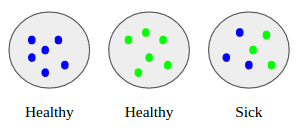
\includegraphics[scale=0.5]{./instance-labels.png}
\caption{This diagram illustrates why static instance labels are not sufficient for phenotype prediction. A patient with 6 of the blue microbe or 6 of the green microbe may be healthy, while a patient with 3 of each is sick. Static instance labels cannot capture this relationship. This is also explained by Amores in his MIL taxonomy \cite{amores13}.} \label{instance-labels}
\end{figure}

\begin{figure}[h]
\centering
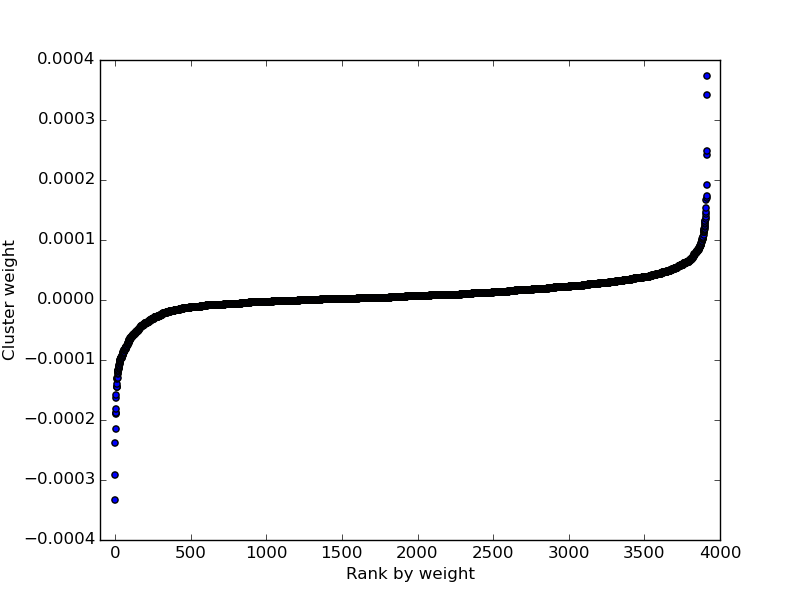
\includegraphics[scale=0.4]{./instance-scatter.png}
\caption{This diagram illustrates the distribution of the instance weights assigned by CAMIL D-BoW. The Y-Axis shows the weights, while the X-Axis shows the ranking of the clusters by weight. Clearly, there are a relatively small number of clusters that have disproportionately large weights, while there is a smaller number of clusters with smaller weights.} \label{instance-scatter}
\end{figure}

One of the benefits of using Multiple Instance Learning methods is that we can attempt to discover instance "labels". In fact, we did not attempt to apply static, unchanging labels to individual reads or clusters, since organisms are affected by their interactions with each other. For instance, a patient with X amount of microbe A or X amount of microbe B may be healthy, but with X/2 amount of microbe A and X/2 amount of microbe B they may be sick. This is illustrated in Figure \ref{instance-labels}. This example is very simplified, but it explains why static instance labels are insufficient.

However, we can infer from the SVM decision boundary which clusters appear to be most relevant to the disease diagnosis. Since feature vectors are multiplied by the weight vector of the decision boundary to determine the label of the patient, we can assume that clusters with the highest weights in the weight vector are most relevant to the disease diagnosis. For instance, if the Ith scalar in the weight vector is has the highest value of any of the weights, then cluster I is likely to play a major role in the disease pathology. Similarly, the most negative weights in the weight vector indicate clusters whose presence in a patient indicates that they likely do not have the disease. Because the data is metagenomic, the clusters represent both phylogenetic and functional similarity, so identifying the most relevant clusters can help discover more about the pathology of the disease. For Type 2 Diabetes, which is a complex phenotype and a disease that is both common and deadly, this is potentially quite valuable.

In the original MGWAS paper, the authors identify 50 important gene markers with mRMR that are used for their classifier. Conversely, CAMIL uses all of the data to train and test the classifier, and subsequently identifies significant clusters based on the classification results. We printed the 25 highest-weighted and 25 lowest-weighted clusters, out of 3188 total clusters. The highest-weighted cluster had a weight of 0.012109, while the lowest-weighted cluster had a weight of -0.003668. The average of the 25 highest cluster weights was 0.010402, while it was -0.002753 for the lowest 25. The average of all 3188 cluster weights was 0.001003, and the median was 0.000254. These results indicate that the highest weights were much larger than the lowest weights and skewed the average weight to be much higher than the median weight. Intuitively, this appears to make sense, as there should be a relatively small number of key clusters whose presence is actually indicative of type 2 diabetes, while most other clusters aren't particularly relevant in this case and whose weights are just noise. Thus, the weights obtained by this method appear to be plausible. In contrast, the labels obtained by GICF were barely differentiated from each other at all. The instance weights determined by CAMIL are shown in Figure \ref{instance-scatter}.